\documentclass[a4paper,12pt]{article}

\usepackage{cmap}					% поиск в PDF
\usepackage[T2A]{fontenc}			% кодировка
\usepackage[utf8]{inputenc}			% кодировка исходного текста
\usepackage[english,russian]{babel}	% локализация и переносы
\usepackage{enumitem}  				% смена типа символя у enumerate
\usepackage{amsmath,amsfonts,amssymb,amsthm,epsfig,epstopdf,titling,url,array}
\usepackage{icomma} 				% "Умная" запятая: $0,2$ --- число, $0, 2$ --- перечисление
\usepackage{hyperref}				% кликабельные ссылки
\usepackage{soulutf8} 				% Модификаторы начертания
\usepackage{mathtools}
\DeclarePairedDelimiter{\ceil}{\lceil}{\rceil}

\usepackage{amstext} % for \text macro
\usepackage{array}   % for \newcolumntype macro
\newcolumntype{L}{>{$}l<{$}} % math-mode version of "l" column type
\newcolumntype{R}{>{$}r<{$}} % math-mode version of "r" column type
\newcolumntype{C}{>{$}c<{$}} % math-mode version of "c" column type


\usepackage[backend=biber,
			bibencoding=utf8,
			maxcitenames=2,
			style=authoryear]	
		{biblatex}					% библиография

\addbibresource{sources.bib}

\newtheorem{theorem}{Теорема}[section]
\newtheorem{corollary}[theorem]{Следствие}


\theoremstyle{definition}
\newtheorem{property}{Свойство}[subsection]
\renewcommand\theproperty{\arabic{property}}

\usepackage[ruled,
			linesnumbered,
			vlined]
		{algorithm2e}				% красивые алгоритмы

\SetAlgorithmName{Алгоритм}{algo}{Список алгоритмов}
\SetKwInput{KwData}{Вход}
\SetKwInput{KwResult}{Выход}
\SetNlSty{textbf}{}{.}
\SetAlgoNlRelativeSize{0}
\SetKwIF{If}{ElseIf}{Else}{Если}{то}{иначе если}{иначе}{}
\SetKwFor{ForEach}{Для каждого}{}{fintq}%
\SetKwFor{While}{Пока}{}{fintq}%


\usepackage[shortcuts]{extdash}

\graphicspath { {img} }

\sloppy

\title{Исследование поточного алгоритма шифрования типа «Раскольников» \linebreak Вариант №4.}
\author{Роман Астраханцев, СКБ-171}

\begin{document}
	\maketitle
	
	\tableofcontents
	
	\section*{Описание алгоритма}

	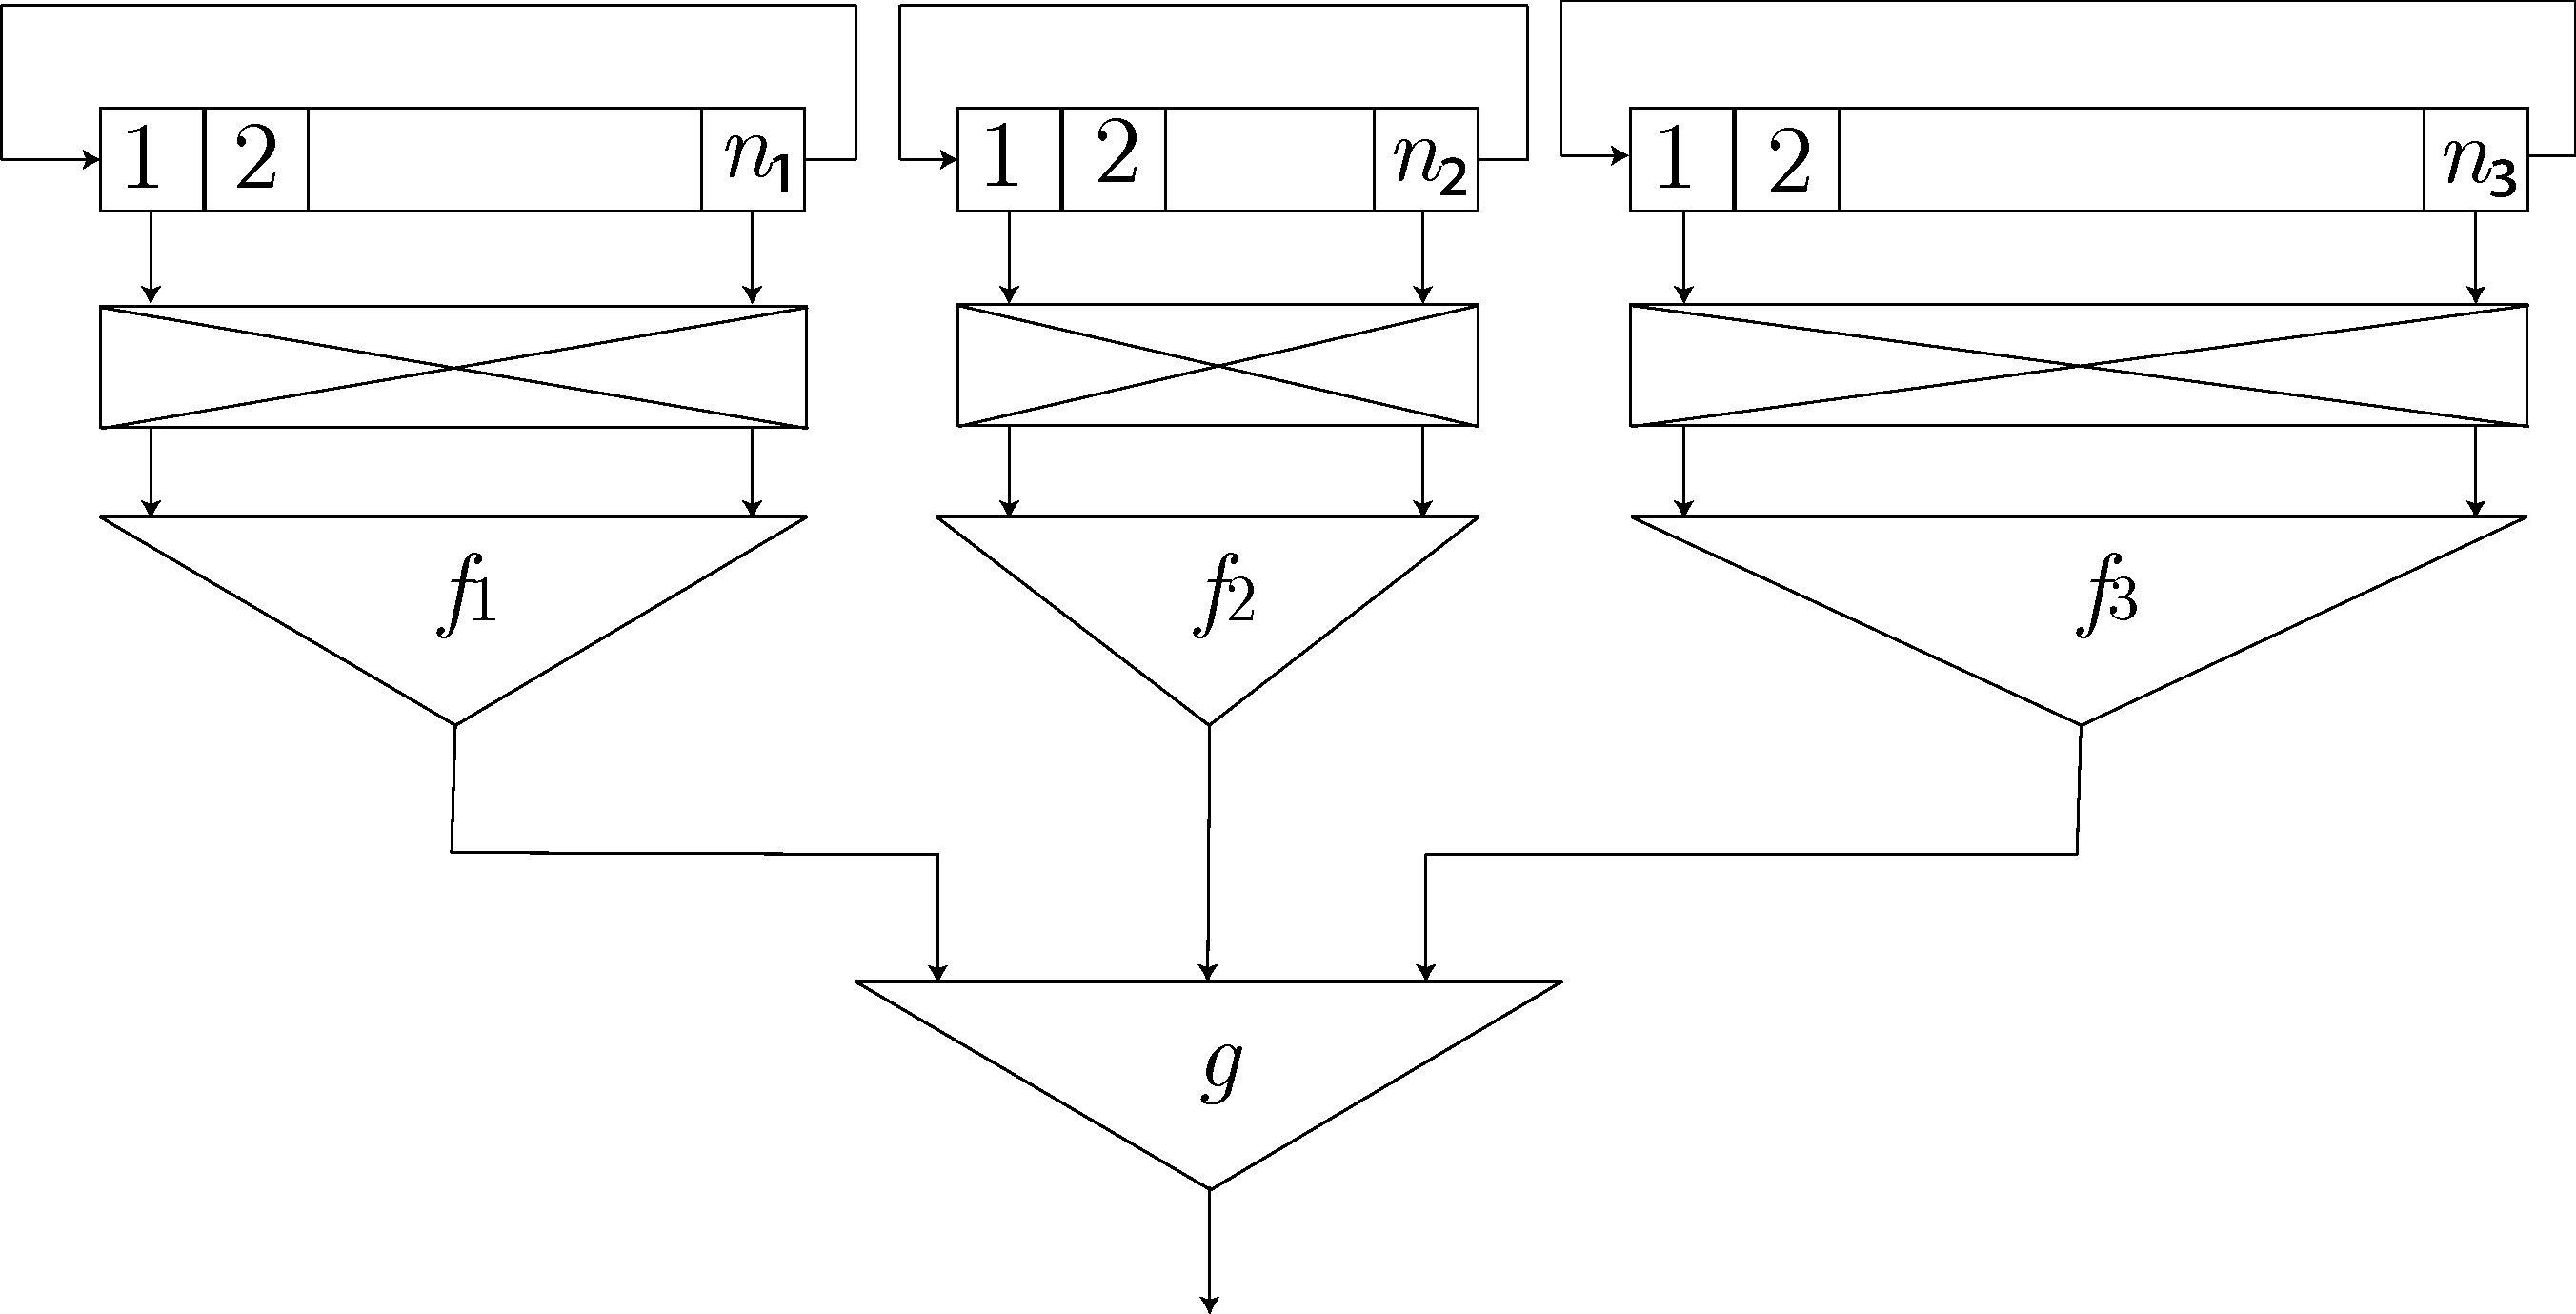
\includegraphics[width=\textwidth]{cipher}

	Поточный алгоритм шифрования типа «Раскольников» состоит из:
	
	\begin{enumerate}
	\item трех РСЛОС $L_i, i \in \overline{1,3}$, над полем $\mathbb{F}_2$ c характеристическими многочленами
	$F_1(x), F_2(x), F_3(x)$ степени соответственно $n_1, n_2, n_3$.
	
	\item трех коммутаторов (перестановок) $K_i, i \in \overline{1,3}, Ki \in S (l_i)$, на вход коммутатору $K_i$
	подаются значения РСЛОС $L_i$ с индексами
	\[ 1 = p_1 < p_2 < \dots < p_{l_i-1} < p_{l_i} = n_i \]

	\item трех функций усложнения выхода РСЛОС $f_i (x_1, x_2, \dots, x_{l_i}), i \in \overline{1,3},$ 
	
	\item комбинирующей булевой функции $g(x,y,z)$, задаваемой формулой ($\land$ -- <<и>>, $\neg$ -- отрицание, $\lor$ -- <<или>>, $\veebar$ -- <<исключающее или>>):
	\[ g(x,y,z) = (\neg x \lor \neg y) \land (x \lor y \lor \neg z) \land (\neg y \lor z) \]
	
	\end{enumerate}

	Ключом являются:
	
	\begin{itemize}[topsep=0pt, itemsep=0pt, parsep=0pt]
	\item начальное заполнение регистра $L_1$
	\item коммутатор $K_2$
	\item начальное заполнение регистра $L_3$
	\end{itemize}

	\section{Исследование ключевого множества}
	
	Множетсво ключей $K$ состоит из всезможожных троек вида $(k_1, k_2, k_3)$, где 
	
	\begin{itemize}[topsep=0pt, itemsep=0pt, parsep=0pt]
	\item $k_1$ - какое-то заполнение регистра $L_1$ длины $n_1$,
	\item $k_2$ - какая-то перестановка длины $n_2$, 
	\item $k_3$ - какое-то заполнение регистра $L_3$ длины $n_1$.
	\end{itemize}
	
	Тогда общее число ключей будет равно
	
	\[ |K| = 2^{n_1} \cdot n_2! \cdot 2^{n_3} \]
	
	Приведём пример параметров $n_1, n_2, n_3$, при котором $|K| > 2^{64}$. Пусть $n_1=25, n_2=10, n_3=25$, тогда
	
	\[ |K| = 2^{25} \cdot 10! \cdot 2^{25} > 2^{25} \cdot 2^{21} \cdot 2^{25} > 2^{71} > 2^{64} \]
	
	\section{Исследование узлов алгоритма}
	
	\subsection{Узлы РСЛОС} \label{Узлы РСЛОС}
	
	\textit{Регистр сдвига с линейной обратной связью} или \textit{РСЛОС} --- это блок, который генерирует двоичные псевдослучайные периодические последовательности, которые называются линейными рекуррентными последовательностями (ЛРП). 
	
	Широкое распространение в криптографических приложениях линейных регистров сдвига над конечными полями $\mathbb{F}_{2^n}$ и кольцами вычетов обусловлено целым рядом факторов. Среди них можно отметить:
	
	\begin{itemize}[topsep=0pt, itemsep=0pt, parsep=0pt]
		\item использование только простейших операций сложения и умножения, аппаратно реализованных практически на всех вычислительных средствах;
		\item высокое быстродействие создаваемых на их основе криптографических алгоритмов;
		\item большое количество теоретических исследований свойств линейных рекуррентных последовательностей (ЛРП), свидетельствующих об их удовлетворительных криптографических свойствах
	\end{itemize}

	В данном шифре в ключ входят только заполнения регистра сдвига, а вид характеристического многочлена, является параметром построения шифра. Значит, нужно подобрать такие функции обратной связи, чтобы для любого \textbf{ненулевого} заполнения ЛРП была максимального периода. В этом нам помогут следующие теормы и следствие из них.
	
	\begin{theorem}
		Пусть $u$ – ЛРП над полем $\mathbb{F}_q$ с реверсивным минимальным многочленом $F(x)$ степени $m$ и $q^m > 2$. Тогда следующие утверждения эквивалентны:
		\begin{enumerate}[topsep=0pt, itemsep=0pt, parsep=0pt, label=(\arabic*)]
			\item $u$ – ЛРП максимального периода;
			\item многочлен $F(x)$ неприводим над $\mathbb{F}_q$, и его корень $\alpha$ в минимальном поле разложения $\mathbb{F}_{q^m}$ над $\mathbb{F}_q$ есть примитивный элемент поля.
		\end{enumerate}
	\end{theorem}

	\begin{theorem}
		Неприводимый многочлен $F(x)$ примитивен в том и только в том случае, когда для любого простого числа $p$, делящего $q^m - 1$, 
		многочлен $x^{\frac{q^m - 1}{p}}$ не сравним с 1 по модулю многочлена $F(x)$.

	\end{theorem}
	
	\begin{corollary}
		Если $F(x)$ -- неприводимый многочлен над полем $\mathbb{F}_2$ степени $m$, и $2^m - 1$ -- простое число, то $F(x)$ -- примитивный многочлен.

	\end{corollary}

	Исходя из утверждений выше, для того чтобы линейная рекуррентная последовательность порядка $m$ над полем из $q$ элементов имела
	максимальный период, необходимо и достаточно, чтобы ее минимальный многочлен был примитивным многочленом.
	
	Более конкретно, над полем $\mathbb{F}_2$ необходимо реверсивный минимальный многочлен $F(x)$ на основе просых чисел Мерсенна. В этом случае для любого \textbf{ненулевого} заполнения ЛРП получается максимального периода.
	
	Приведём конкретный пример многочленов $F_1(x), F_2(x), F_3(x)$ для заданных нашим алгоритмом РСЛОС $L_1, L_2, L_3$. Для их генерации будем использовать втроенные функции пакета Wolfram Mathematica 
	
	Пусть $n_1=31, n_2=13, n_3=19$ ($2^{31}-1, 2^{13}-1$ и $2^{19}-1$ --- это известные числа Мерсенна).
	
	Пример неприодимых многочленов соотвествующих степеней из $\mathbb{F}_2$[x].
	\begin{align*}
		F_1(x) =& x^{31} + x^{30} + x^{29} + x^{28} + x^{27} + x^{24} + x^{21} + x^{19} + \\
			    &+ x^{18} + x^{13} + x^{12} + x^{10} + x^4 + x^3 + 1 \\[2ex]
		F_2(x) =& x^{13} + x^{12} + x^{11} + x^8 + x^7 + x^6 + x^5 + x^4 + x^2 + x + 1 \\[2ex]
		F_3(x) =& x^{19} + x^{15} + x^{13} + x^{12} + x^{10} + x^9 + x^5 + x^4 + x^2 + x + 1 
	\end{align*}
	
	В этом случае любое \textbf{ненулевое} заполнение каждого из $L_1, L_2, L_3$ даст нам максимальный период на каждом из регистрах. Кроме того, каждый регистр сдвига был выбран разной длинны для того, чтобы исключить случай совместного зацикливания двух ЛРП. Иными словами итоговый период совместной работы всех трёх регистров будет равна 
	
	\[ N_{L_1 L_2 L_3} = \text{НОК}(2^{n_1}-1, 2^{n_2}-1, 2^{n_3}-1) = \text{НОК}(2^{31}-1, 2^{13}-1, 2^{19}-1) \approx 2^{63} \]

	Это означает, что вектор начальных заполнений $(u_1, u_2, u_3)$ регистров $L_1, L_2, L_3$ вернётся в сам в себя после $N_{L_1 L_2 L_3} \approx 2^{63} $ совместных тактов работы всех трёх регистров.
	
	При этом мощность ключевого множества по-прежнему будет удовлетворять условию $|K| > 2^{64}$:
	
	\[ |K| = 2^{31} \cdot 13! \cdot 2^{19} > 2^{31} \cdot 2^{32} \cdot 2^{19} > 2^{82} > 2^{64} \]
	
	\subsection{Функции усложнения} \label{Функции усложнения}
	
	Для усложнения аналитической сложности выходной	последовательности РСЛОС используются функции усложнения. «Фильтрующая» функция f должна выбираться так, чтобы выходная последовательность имела распределение, близкое к равномерному распределению, и высокую линейную сложность.

	
	Ниже представленые основные криптографические характеристики нелинейных преобразований, используемые в поточных шифрах.
	
	
	\begin{property}
		Функция $f$ фильтрующего генератора должна быть сбалансированной, т.е.  $|\{x : f(x) = 0\}| = 2^{n-1} $.  
	\end{property}

	\begin{property} \label{prop::zapr}
		У функция $f$ фильтрующего генератора должны отсуствовать запреты. 
	\end{property}

	Для выполненеия свойтсва \ref{prop::zapr} достаточно, чтобы функция $f$ была линейна по крайней переменной. Есть более общий критерий определения имеет ли булева фунция запрет или нет.
	
	\begin{theorem}
		Булева функция не имеет запрета тогда и только тогда, когда она сильно равновероятна.

	\end{theorem}

	\begin{property} 
		У функция $f$ фильтрующего генератора должна иметь высокую алгебраическую степень.
	\end{property}

	\begin{property} 
		Функция $f$ фильтрующего генератора должна иметь высокую нелинейность, т.е. не иметь эффективных линейных статистических аналогов.
	\end{property}

	\begin{property} 
		Функция $f$ фильтрующего генератора должна быть $k$\-/равновероятной для максимально возможного значения $k$.
	\end{property}
	
	\begin{property} 
		Функция $f$ фильтрующего генератора (а также функция $f~+~1$) не должны иметь аннигиляторов малой алгебраической степени.
	\end{property}
	
	
	На практикте помимо достежния перечисленных условий необходимо дополнительно исследовать весь блок фильтрующего гереатора целиком.
	Например, фильтрующий генератор с нелинейной функцией усложнения может представляться в виде ЛРП с меньшим (чем исходная ЛРП) периодом.
	
	В работе \textcite{rachwalik2012generation} были найдены несколько функций усложнения порядков 25 и 27. Работа была нацелена на поиск таких фукнций, что обеспечивают наибольший период выходной последовательности. Кроме того у перечисленных в работе булевых функций были ислледованы некоторые статистические свойства выходных последовательностей. Возьмём эти функции усложнения за основу, приняв некоторые переменные за единицу.
	
	\begin{align*}
		f_1 =& x_0 \oplus x_6 \oplus x_{11} \oplus x_{14} \oplus x_{16} \oplus x_{17} \oplus x_{18} \oplus x_{19} \oplus x_{23} \oplus\\
			 &\oplus x_{4} x_{19} \oplus x_{4} x_{21} \oplus x_5 x_{22} \oplus x_9 x_{19} \oplus x_1 x_{17} x_23 \oplus x_5 x_7 x_{18} \oplus x_5 x_{12} x_{19} \\[2ex]
		f_2 =& x_0 \oplus x_3 \oplus x_6 \oplus x_{10} \oplus x_6 x_9 \oplus x_6 x_{10} \oplus x_4 x_9 x_{10} \\[2ex]
		f_3 =& x_0 \oplus x_8 \oplus x_9 \oplus x_{10} \oplus x_{11} \oplus x_{10} x_{14} \oplus x_4 x_{16}\oplus x_{11} x_{16} \oplus x_1 x_5 x_7 
	\end{align*}
	
	\subsection{Комбинирующая функция}
	
	\subsubsection{Вычисление многочлена Жегалкина}
	
	С помощью быстрого преобразования Фурье вычислим коэффициенты многолчена Жегалкина для булевой функции $g$.
	
	\begin{table}[h!]
		\begin{center}
			\begin{tabular}{|c|c|c|c||c||c|c|c|}
				\hline
				\textbf{Моном} & $ \pmb{x} $ & $ \pmb{y} $ & $ \pmb{z} $ & $ \pmb{g} $ & $ \pmb{g_1} $ & $ \pmb{g_2} $ & $ \pmb{g_3} $ \\ \hline
				1 & 0 & 0 & 0 & 1 & 1 & 1 & 1 \\ \hline
			  $z$ & 0 & 0 & 1 & 0 & 1 & 1 & 1 \\ \hline
			  $y$ & 0 & 1 & 0 & 0 & 0 & 1 & 1 \\ \hline
			$y z$ & 0 & 1 & 1 & 1 & 1 & 0 & 0 \\ \hline
			  $x$ & 1 & 0 & 0 & 1 & 1 & 1 & 0 \\ \hline
			$x z$ & 1 & 0 & 1 & 1 & 0 & 0 & 1 \\ \hline
			$x y$ & 1 & 1 & 0 & 0 & 0 & 1 & 0 \\ \hline
		  $x y z$ & 1 & 1 & 1 & 0 & 0 & 0 & 0 \\ \hline
			\end{tabular}
		\end{center}
	\end{table}
		
	В итоге получаем 	
	\[ g(x,y,z) = 1 \oplus y \oplus z \oplus x z\]
	
	

	\subsubsection{Характеристики} \label{Характеристики}
	
	Вычислим характерсики комбинирующей функции, которые позволят нам определить возможность применения разлинчых методов атак.
	
	Из вида многочлена жегалкина видно, что \textbf{степень нелинейности} функции $g$ равна 2. 
	
	Булева функция $h = x y$ является \textbf{аннигилятором} функции $g$, поскольку
	\[ h g = \left(1 \oplus y \oplus z \oplus x z \right) xy = xy \oplus xy \oplus xyz \oplus xyz = 0 \]

	Из предыдущего пункта видно, что \textbf{вес} функции $|g(x,y,z)| = 4$. Это означает, что функция $g$ является \textbf{сбалансированной} (равновероятной)
	
	\[ P(g = 0) = \frac{4}{8} = P(g = 1) \]

	Исследуем функцию $g$ на корреляционную иммунность. Для этого будет поочерёдно фиксировать значения переменных и считать вероятность получения $0$ до тех пока она не станет отличной от $0.5$.
	
	\begin{align*}
		P\bigl( g(x,y,z) = 0\ |\ x = 0\bigr) &= P(1\oplus y \oplus z = 0) = \frac{1}{2} \\ 
		P\bigl( g(x,y,z) = 0\ |\ x = 1\bigr) &= P(1\oplus y = 0) = \frac{1}{2} \\[2ex]
		P\bigl( g(x,y,z) = 0\ |\ y = 0\bigr) &= P(1 \oplus z \oplus x z\ = 0) = \frac{3}{4} \\ 
		P\bigl( g(x,y,z) = 0\ |\ y = 1\bigr) &= P(z \oplus x z = 0) = \frac{1}{4} \\[2ex]
		P\bigl( g(x,y,z) = 0\ |\ z = 0\bigr) &= P(1 \oplus y = 0) = \frac{1}{2} \\ 
		P\bigl( g(x,y,z) = 0\ |\ z = 1\bigr) &= P(y \oplus x = 0) = \frac{1}{2} 
	\end{align*}
	
	Из вычислений выше видно, что фиксация переменной $y$ вероятность отклоняется от исходной. А значит функция $g$ \textbf{не} является \textbf{корреляционно-иммунной}.

	Вспомним, что произвольная булева функция $f$ является $k$-устойчивой тогда и только тогда, когда она корреляционно-иммунная порядка $k$ и равновероятна. Из рассуждений выше следует, что функция $g$ также \textbf{не} является \textbf{устойчивой}.
	
	Исследуем функцию $g$ на наличие запретов. Для этого в пакете Wolfram Mathematica будем перебирать всевозможные выходные последосвательности разной длинны и пытаться решить систему уравнений относительно ячеек регистра сдвига. В результате такого исследования были найдены следующие невозможные выходные гаммы.
	
	\begin{align*}
		&001000\dots  & &1001000\dots\\
		&111000\dots  & &0111000\dots\\
		&0001000\dots & &1111000\dots 
	\end{align*}

	Из наличия запретов следует, что функция $g$ \textbf{не} является \textbf{сильноравновероятной}.
	

	\subsubsection{Наилучшее приближение линейной функцией} \label{Наилучшее приближение линейной функцией}
	
	С помощью быстрого преобразования Фурье вычислим наилучшее приближение для булевой функции $g$.
	
	\begin{table}[h!]
		\begin{center}
			\begin{tabular}{|c|c|c|c||c||c|c|c|}
				\hline
				\textbf{Многочлен} & $ \pmb{x} $ & $ \pmb{y} $ & $ \pmb{z} $ & $ \pmb{g} $ & $ \pmb{g_1} $ & $ \pmb{g_2} $ & $ \pmb{g_3} $ \\ \hline
					1 & 0 & 0 & 0 & 1 &  1/2 &  1/2 &  1/2 \\ \hline
				  $z$ & 0 & 0 & 1 & 0 &  1/2 &    0 &    0 \\ \hline
			   	  $y$ & 0 & 1 & 0 & 0 &  1/2 &    0 &  1/4 \\ \hline
		 $y \oplus z$ & 0 & 1 & 1 & 1 & -1/2 &  1/2 &  1/4 \\ \hline
				  $x$ & 1 & 0 & 0 & 1 &    1 &  1/2 &    0 \\ \hline
		 $x \oplus z$ & 1 & 0 & 1 & 1 &    0 &    0 &    0 \\ \hline
		 $x \oplus y$ & 1 & 1 & 0 & 0 &    0 &  1/2 & -1/4 \\ \hline
$x \oplus y \oplus z$ & 1 & 1 & 1 & 0 &    0 &    0 &  1/4 \\ \hline
			\end{tabular}
		\end{center}
	\end{table}

	TO DO

	В итоге получаем, что булева функция	
	\[ \tilde{g}(x,y,z) = x \oplus y \oplus z \]
	является наилучшим линейным приближением булефой фукнции $g$. Посчитаем вероятность того, что значения этих функций совпали.
	
	\[ p(g=\tilde{g}) = \frac{3}{4} \]
	
	\subsubsection{Строгий лавинный критерий}
	
	Исследуем насколько сильно изменяются значения булевой функции $g(x, y, z)$ при малом изменении значений входных переменных. Для этого расчитаем производые по направлениям координатных веторов в $V_3$
	
	
	\begin{table}[h!]
		\begin{center}
			\begin{tabular}{|c|c|c||c||c|c|c|}
				\hline
				$ \pmb{x} $ & $ \pmb{y} $ & $ \pmb{z} $ & $ \pmb{g} $ & $ \pmb{D_x g} $ & $ \pmb{D_y g} $ & $ \pmb{D_z g} $ \\ \hline
				0 & 0 & 0 & 1 & 0 & 1 & 1 \\ \hline
				0 & 0 & 1 & 0 & 1 & 1 & 1 \\ \hline
				0 & 1 & 0 & 0 & 0 & 1 & 1 \\ \hline
				0 & 1 & 1 & 1 & 1 & 1 & 1 \\ \hline
				1 & 0 & 0 & 1 & 0 & 1 & 0 \\ \hline
				1 & 0 & 1 & 1 & 1 & 1 & 0 \\ \hline
				1 & 1 & 0 & 0 & 0 & 1 & 0 \\ \hline
				1 & 1 & 1 & 0 & 1 & 1 & 0 \\ \hline
			\end{tabular}
		\end{center}
	\end{table}
	
	
	Таблица выше демонстирует, что производная по направлению $y$ \textbf{не сбалансирована}. Это значит, что булева функция $g$ \textbf{не} удовлетворяет \textbf{строгому лавинному критерию}. Более того, это означает что булева функция $g$ \textbf{не удовлетворяет критерию распространения}.
	
	\section{Методы восстановления ключа}
	
	Зафиксируем параметры согласно размышлениям из пунктов \ref{Узлы РСЛОС} и \ref{Функции усложнения} и исследуем применимость разных методов для восстановления ключа. Для каждого алгоритма вычислим его характеристики.
	
	
	\subsection{Метод тотального опробования}
	
	Самым наивным вариантом восстановления ключа будет алгоритм тотального опробования, который применим абсолютно к любому шифру. Идея алготима заключается в переборе всевозможных ключей и сопоставлении полученной гаммы с известным материалом.
	
	Через $G(K, n)$ будем обозначать выработку гаммы $\Gamma$ длинны $n$ представленным поточным алгоритмом шифрования на ключе $K$. Количество материала, необходимое для однозначного определения ключа составляет $m=\ceil{\log_2(|K|)}=83$ бита.

	\begin{algorithm}[H]
		
		\caption{Метод тотального опробования}
		\label{alg:Total}
		\SetAlgoNoEnd
		
		\KwData{Пара открытый и шифрованный текст $P, C \in V_{83}$}
		\KwResult{Ключ шифрования $K$}
		
		\ForEach{$k_1 \in V_{31}$}{ 
			\ForEach{$k_2 \in S (13)$}{ 
				\ForEach{$k_3 \in V_{19}$}{ 
					Сформировать ключ $K=(k_1, k_2, k_3)$
					
					Вычислить $\Gamma = G(K, 83)$ \\
					\If{$P \oplus C = \Gamma$,}{
						Закончить алгоритм и вернуть $K$
					}
				}
			}
		}
	\end{algorithm}	
	
	
	\textbf{Вероятность работы} алгоритма $p(A)=1$, поскольку алгоритм гарантированно находит ключ. 
	
	\textbf{Средняя трудоёмкость} алгоритма $S(A)=\frac{2^{31} \cdot 13! \cdot 2^{19} + 1}{2} \approx 2^{82} $ использований алгоритма выработки гаммы. Она же равна \textbf{трудоёмкости по Шеннону} $Q(A)$.
	
	\textbf{Объём памяти} необходимый для работы алгоритма $M(A) = O(1)$ бит, поскольку алгоритм хранит только локальные переменные.
	
	\subsection{Метод встречи по середине}
	
	Прежде чем применить метод встречи по середине, необходимо представить преобразование исходного шифра как двойное последовательное шифрование. Иными словами если алгоритм зашифрования $E_K(P)$ открытого текста $P$ на ключе $K$ можно представить в виде $E'_{k_1}(E''_{k_2}(P))$, то можно применить метод встречи по середине. Наример, выход булевой функции $g(x,y,z) = 1 \oplus y \oplus z \oplus x z$, где $x, y, z$ - выходы фильтрующих функций соответсвующих блоков шифра, может быть представлен, как сложение двух булевых функций $ h_1=1 \oplus y $ и $ h_2=z \oplus x z $. 
	
	Наиболее эффективным с точки зрения трудоёмкости этот метод становится тогда, когда алгоритм зашифрования $E_k(P)$ удалось представить в виде $E'_{k_1}(E''_{k_2}(P))$ так, что длина $k_1$ $\approx$ длине $k_2$.
	
	Теоретически блок коммутатора (перестановка) $K_2$ можно было бы разделить на 2 блока коммутатора меньшей длины с общим входом. Поскольку блок РСЛОС не является ключевым, то он может быть задан ввиде таблицы.
	
	Однако для упрощения рассмотрим разделение так, что $E'_{k_1}$ -- это центральный блок, а $E''_{k_2}$ -- это правый и левый блоки. Для однознчаного отделения ключа $k_2$ достаточно $33$ бит материала, иными словами исходный материал (83 бита) разделить как 33 и 50 бит соответсвенно.
	
	Разделим исходный алгоритм шифрования $E_K(P)$, где $P$ -- открытый текст длины $n$ и напишем текст работы алгоритма.

	\begin{multline*}	
	E_K(P) = P \oplus G(K, n) = \\ = P \oplus g(x,y,z) = (P \oplus 1 \oplus y) \oplus z \oplus x z = E''_{k_2}(P) \oplus z \oplus x z = \\ = E'_{k_1}(E''_{k_2}(P))
	\end{multline*}
	
	\begin{algorithm}[H]
		
		\caption{Метод встречи по середине}
		\label{alg:Midle}
		\SetAlgoNoEnd
		
		\KwData{Пара открытый и шифрованный текст $P, C \in V_{83}$}
		\KwResult{Ключ шифрования $K$}
		
		Разделить исходный материал на $P_1, C_1 \in V_{33}$ и $P_2, C_2 \in V_{50}$
		
		\ForEach {$k_2 \in S (13)$}{ 
			
			Вычислить П$= E''_{k_2} (P_1)$
			
			Занести в ячейку с адресом П ключ $k_2$

			\tcc{в среднем в каждой ячейке памяти будет лежать около 1 ключа}
		}

		\ForEach{$k_1 \in V_{31}$}{ 
			\ForEach{$k_3 \in V_{19}$}{ 
				Сформировать ключ $\tilde{k}_1=(k_1, k_3)$
				
				Вычислить П$= E'^{-1}_{k_1} (C_1)$

				\If{ячейка с адресом П не пуста}{
					Достать из неё ключ $k_2$
					
					Сформировать ключ $K=(k_1, k_2, k_3)$
					
					Доопробовать ключ $K$ на материале $P_2, C_2$
					
					\If{доопробование успешно}{
						Закончить алгоритм и вернуть $K$
					}
				}				 
			}
		}
	
	\end{algorithm}	
	
	
	\textbf{Вероятность работы} алгоритма $p(A)=1$, поскольку алгоритм гарантированно находит ключ. 
	
	\textbf{Средняя трудоёмкость} алгоритма $S(A)= 13! \cdot s_1 + \frac{2^{31} \cdot 2^{19} + 1}{2} \cdot s_2 $, где $s_1$ -- сложность алготима зашифрования $E''$, $s_2$ -- сложность алготима расшифрования $E'^{-1}$ . Средняя трудоёмкость равна \textbf{трудоёмкости по Шеннону} $Q(A) = S(A) \approx 2^{33} \cdot s_1 + 2^{49} \cdot s_2$.
	
	\textbf{Объём памяти}, который необходим необходимый для успешной работы алгоритма $M(A) = 2^{33} \cdot 13! + O(1) \approx 2^{66} + O(1)$ бит, поскольку алгоритму требуется хранить таблицу ключей из $S(13)$. Для описания одного ключа из $S(13)$ требуется 33 бита ($2^{33}$ -- это размерность пространства памяти). Поэтому в среднем будет в каждой 33-битной ячейке памяти будет храниться не более одного ключа. К сожалению, в современных реалиях хранение таблицы размером $2^{66}$ бит не представляется возможным.
	

	\subsection{Стетистический метод}
	
	В основе статистического метода лежит построение некоторой статистики, на которой строится предположение о правильности ключа или его части. Если эта статистика превышает неоторый статистический порог $T$ (который зависит от $\alpha$ и $\beta$, статистических ошибок 1-го и 2-го рода соотвественно), то можно с вероятностью $p=1-\alpha$ полагать, что ключ или его часть подобраны верно.
	
	В пункте \ref{Характеристики} было отмечено, что комбинирующая функция $g$ не обладает корреляционной имунностью, а в подпункте \ref{Наилучшее приближение линейной функцией} был найден линейный статистический аналог функции $g$, вероятность совпадения с котрым больше $1/2$. Это позволяет провести атаку либо с использованием \textbf{корреляционного метода}, либо с ипользваонием \textbf{линейного статистического аналога}. Рассмотрим статистический метод на примере корреляционной зависимости.
	
	Вспомним, что 
	\[ p(g= \bar{y}) = \frac{6}{8} = \frac{3}{4} \]
	Это означает, что можно построить такую статистику, которая бы отражала корреляционную зависимость выходов гаммы и центрального блока. Функция корреляции последовательностей $\{\gamma_i\}_{i=1}^N$ и $\{\theta_i\}_{i=1}^N$ длины $N$
	
	\[  C(\gamma, \theta) = \sum_{i=1}^{N} \left(-1\right)^{\gamma_i +\theta_i} \]
	
	Наблюдение выше позволяет использовать выход последовательности центрального блока, как индикатор того, коррелирует ли с ней выходная гамма всего шифра. Идея метода заключается в том, чтобы для всевозможных ключей центрального блока вырабатывать выходные значения этого блок и считать функцию корреляции между полученной и взламываемой гаммой. Если эта функция превышает неоторый статистический порог $T$ (который зависит от длины $N$ выработанной гамммы и $\alpha$ и $\beta$, статистических ошибок 1-го и 2-го рода соотвественно), то можно с вероятностью $p=1-\alpha$ полагать, что ключ центрального блока подобран верно.

	\textbf{Количество материала} в данном случае состоит из двух частей: материал для статистического исследвания корреляции и материал для доопробования. Чем больше будет матриала для статистического исследвания, тем точнее покажет себя алгоритм, поэтому примем это $N$, количество бит, за параметр алгоритма. Материал же для доопробования можно полгадать равным 50 бит (достаточным для однозначного определения ключа).
	
	Обозначим за $G'(k, n)$ выработу гаммы длины $n$ центальным блоком на ключе $k$.
	
	\begin{algorithm}[H]
		
		\caption{Корреляциооный метод}
		\label{alg:Corr}
		\SetAlgoNoEnd
		
		\KwData{Пары открытый и шифрованный текст $P_1, C_1 \in V_{N}, P_2, C_2 \in V_{50}$}
		\KwResult{Ключ шифрования $K$}
		
		Вычислить последовательность $\gamma = P_1 \oplus C_1$
		
		\ForEach {$k_2 \in S (13)$}{ 
			
			Вычислить последовательность $\theta = G'(k_2, N)$
			
			Вычилсить $C=C(\gamma, \theta)$
			
			\If{C > T}{
				\ForEach{$k_1 \in V_{31}$}{ 
					\ForEach{$k_3 \in V_{19}$}{ 
						Сформировать ключ $K=(k_1, k_2, k_3)$
							
						Доопробовать ключ $K$ на материале $P_2, C_2$
							
						\If{доопробование успешно}{
							Закончить алгоритм и вернуть $K$
						}
					}
				}	
			}	
		}
	\end{algorithm}	
	
	Как уже отмечалось ранее \textbf{вероятность работы} алгоритма $p(A)=1-\alpha$, где $\alpha$ -- это статистическая ошибка 1-го рода, зависящая от $N$. 
	
	\textbf{Средняя трудоёмкость} алгоритма при выбранных $\alpha$ и $\beta$ 
	\begin{multline*}	
	S(A)=\left( 1-\alpha \right)\cdot \left( \frac{13! + 1}{2} \cdot N + \beta \frac{13! + 1}{2} \frac{2^{31} \cdot 2^{19} + 1}{2} \right) + \\ + \alpha \left( 13! \cdot N + \beta \cdot 2^{31} \cdot 2^{19}  \right).
	\end{multline*}		

	\textbf{Объём памяти} необходимый для работы алгоритма $M(A) = O(1)$ бит, поскольку алгоритм хранит только локальные переменные.
	
	Стоит так же отметить, что на этапе доопробоваия для нахождения отсавшейся части ключа также, можно использовать разные методы. Например, успешное использование метода встречи по середине может уменьшить среднюю трудоёмкость до $O\left(N\cdot\left( 2^{33} + 2^{31} + 2^{19} \right) \right)$
	
	\subsection{Метод частичного опробования с ипользованием аннигилятора}
	
	В пункте \ref{Характеристики} было замечено, что функия $h=x y$ является аннигилятором комбинирующей функции $g$. Заметим, что функция $h$ зависти только от выходов левого и центального блоков. Это означает, что на позициях, где выходная гамма равна 1, значение функции $h=0$ (из определения аннигилятора). Это позволяет успешно воспользоваться \textbf{методом частичного опробования}.
	
	Перебирая всевозможные ключи левого и центрального блока мы можем определить является ли совместный ключ двух блоков валидным, если на всех позициях, где выходная гамма равна 1 функция $h$ равна нулю. Стоит заметить, что для успешного применения метода достаточно 83 бит \textbf{материала} с тем условием, что среди них будет 64 бита будут единицами.
	
	Будем обозначать через $G_x(K_x, n)$ и $G_y(K_y, n)$ вычисление $n$ бит выходной гаммы левого и центрального блоков соотвественно.
	
	
	\begin{algorithm}[H]
		
		\caption{Метод частичного опробования с ипользованием аннигилятора}
		\label{alg:Annig}
		\SetAlgoNoEnd
		
		\KwData{Пары открытый и шифрованный текст $P, C \in V_{83}$}
		\KwResult{Ключ шифрования $K$}
		
		Вычислить $\Gamma = P \oplus C $ 
		
		\ForEach{$k_1 \in V_{31}$}{ 
			
			Вычислить $\Gamma_x = G_x(k_1, 83)$
			
			\ForEach{$k_2 \in S(13)$}{ 
				
				Вычислить $\Gamma_y = G_y(k_2, 83)$
				
				Вычислить $\Gamma_{x y} = \Gamma_x\ \&\ \Gamma_y $
				
				Проверить, что на всех местах, где в последовтальности $\Gamma$ стоят единицы в последовательности $\Gamma_{x y}$ стоят нули.
				
				\If{проверка успешна}{
					
					\ForEach {$k_3 \in V_{19}$}{ 
						
						Сформировать ключ $K=(k_1, k_2, k_3)$
						
						Доопробовать ключ $K$ на материале $P, C$
						
						\If{доопробование успешно}{
							Закончить алгоритм и вернуть $K$
						}
					}
				}
			}
		}		
	\end{algorithm}	

	\textbf{Вероятность работы} алгоритма $p(A)=1$, поскольку алгоритм гарантированно находит ключ. 
	
	\textbf{Средняя трудоёмкость} алгоритма $S(A)= \frac{2^{31} \cdot 13! + 1}{2} s_1 + \frac{2^{19} + 1}{2} s_2$, где $s_1$ -- сложность алготима выработки гаммы $\Gamma_{x y}$ и проверки согласованности её с материалом, $s_2$ -- сложность алготима доопробования. 
	
	Средняя трудоёмкость равна \textbf{трудоёмкости по Шеннону} $Q(A) = S(A) \approx 2^{63} \cdot s_1 + 2^{18} \cdot s_2$.
	
	\textbf{Объём памяти} необходимый для работы алгоритма $M(A) = O(1)$ бит, поскольку алгоритм хранит только локальные переменные.
	
	\section{Выводы и рекомендации}
	
	Из разобранных методов для восстановления ключа лучше всего подходят \textbf{корреляционный метод} и \textbf{метод частичного опробования с ипользованием аннигилятора}. В зависимости от количества материала или имеющихся вычислительных мощностей можно отдать предпочтение одному или другому методу. 
	
	Для повышения стойкости алгоритма шифрования стоит выбрать более стойкую комбинирующую функцию. А именно, стоит выбрать функцию $g(x,y,z)$, аннигилятор которой зависит от всех выходных блоков. Также стоит гаранитровать корреляционную имунность хотя бы 1 порядка. Кроме того универсальным способом увеличения стойкости алгоритма является увеличение мощности ключевого множества за счёт увеличения длины регистров РСЛОС.
			
\end{document}